% !Mode:: "TeX:UTF-8"
% !TEX program  = xelatex

%\documentclass{cumcmthesis}
\documentclass[withoutpreface,bwprint]{cumcmthesis} %去掉封面与编号页

\usepackage{url}   % 网页链接
\usepackage{cases}
\usepackage{subcaption} % 子标题
\title{全国大学生数学建模竞赛编写的 \LaTeX{} 模板}
\tihao{A}
\baominghao{4321}
\schoolname{XX大学}
\membera{}
\memberb{向左}
\memberc{哈哈}
\supervisor{老师}
\yearinput{2017}
\monthinput{08}
\dayinput{22}

\title{二维非齐次热传导方程的向后Euler ADI格式}
\begin{document}
	\maketitle
	~\\
	~\\
	
	作业:
	
	$$
	\left\{
	\begin{array}{lcl}
	\dfrac{\partial{u}}{\partial{t}}-(\dfrac{\partial^{2}{u}}{\partial{x}^{2}}+\dfrac{\partial^{2}{u}}{\partial{y}^{2}})=- \dfrac{3}{2}e^{\frac{1}{2}(x+y)-t} &,&0 < x,y < 1,0 < t \leq 1 \\
	
	u(x,y,0)=e^{\frac{1}{2}x-t} &, & 0 < x,y < 1 \\
	
	u(0,y,t)=e^{\frac{1}{2}y-t},u(1,y,t)=e^{\frac{1}{2}(1+y)-t},&, &0 \leq y \leq 1,0 \leq t \leq 1 \\
	
	u(x,0,t)=e^{\frac{1}{2}x-t},u(x,1,t)=e^{\frac{1}{2}(1+x)-t},&, &0 < x < 1,0 \leq t \leq 1 
	\end{array}
	\right.
	$$

该问题的精确解为$ u(x,y,t)=e^{\frac{1}{2}(x+y)-t}$.

定义误差为$$ E_{\infty}(h,\tau)=\max \limits_{1 \leq i,j \leq m-1 \atop 1 \leq k \leq n } |u_{i,j}^k-u(x_i,y_j,t_k)| $$

用向后Euler ADI格式求下述问题的数值解并对数值解、精度和误差阶进行相应的数值分析。


~\\
~\\

解:

将x和y  m等分,将t  n等分, 记$h=\dfrac{1}{m},\tau=\dfrac{1}{n}$

$x_i=ih,0 \leq i \leq m$
$y_j=jh,0 \leq j \leq m$
$t_k=k \tau,0 \leq k \leq n$

差分格式为
%\begin{subequations}
%\begin{numcases}{}
%	3x+4y=5\\
%	5x-9y=13
%\end{numcases}
%\end{subequations}

\begin{subequations}
	\begin{numcases}{}
		(I-\tau \delta_x^2)u_{i,j}^{k+\frac{1}{2}}=u_{i,j}^{k}+\tau f_{i,j}^{k+1} \\
		\label{1a}
		(I-\tau \delta_y^2)u_{i,j}^{k+1}=u_{i,j}^{k+\frac{1}{2}}
		\label{1b}
	\end{numcases}
\end{subequations}

其中
$Iu_{i,j}^k=u_{i,j}^k$,$u_{i,j}^{k+\frac{1}{2}}$为中间层。
$\delta_x^2u_{i,j}=\dfrac{u_{i+1,j}-2u_{i,j}+u_{i-1,j}}{h^2}.$
$\delta_y^2u_{i,j}=\dfrac{u_{i,j+1}-2u_{i,j}+u_{i,j-1}}{h^2}.$


(1a)可以写成矩阵形式

$$A u_{i,j}^{k+\frac{1}{2}}=B_1^{k+1}$$.

$$
A=
\begin{bmatrix}
	1+2\gamma & -\gamma \\
	-\gamma & 1+2\gamma & -\gamma \\
	& \ddots & \ddots & \ddots \\
	& & 	-\gamma & 1+2\gamma
\end{bmatrix}
$$

$$
B_1^{k+1}=[u_{1,j}^k,u_{2,j}^k,\cdots,u_{m-1,j}^k]^T+\tau [f_{1,j}^{k+1},f_{2,j}^{k+1},\cdots,f_{m-1,j}^{k+1}]^T+ \gamma[u_{0,j}^{k+\frac{1}{2}},0,\cdots,0,u_{m,j}^{k+\frac{1}{2}}]^T.
$$

(\ref{1b})可写成矩阵形式

$$A u_{i,j}^{k+\frac{1}{2}}=B_2^{k+1}$$.
$$
B_2^{k+1}=[u_{i,1}^{k+\frac{1}{2}}+\gamma u_{i,0}^{k+1},u_{i,2}^{k+\frac{1}{2}},\cdots,u_{i,m-2}^{k+\frac{1}{2}},u_{i,m-1}^{k+\frac{1}{2}}+\gamma u_{i,m}^{k+1}]^T
$$

~\\
~\\




\textbf{解题程序运行于Matlab 2018a}

$\tau=\dfrac{1}{10},h=\dfrac{1}{10}$时t=1处的数值解和精确解见图\ref{fig:f1},非常接近。
\begin{figure}
	\centering
	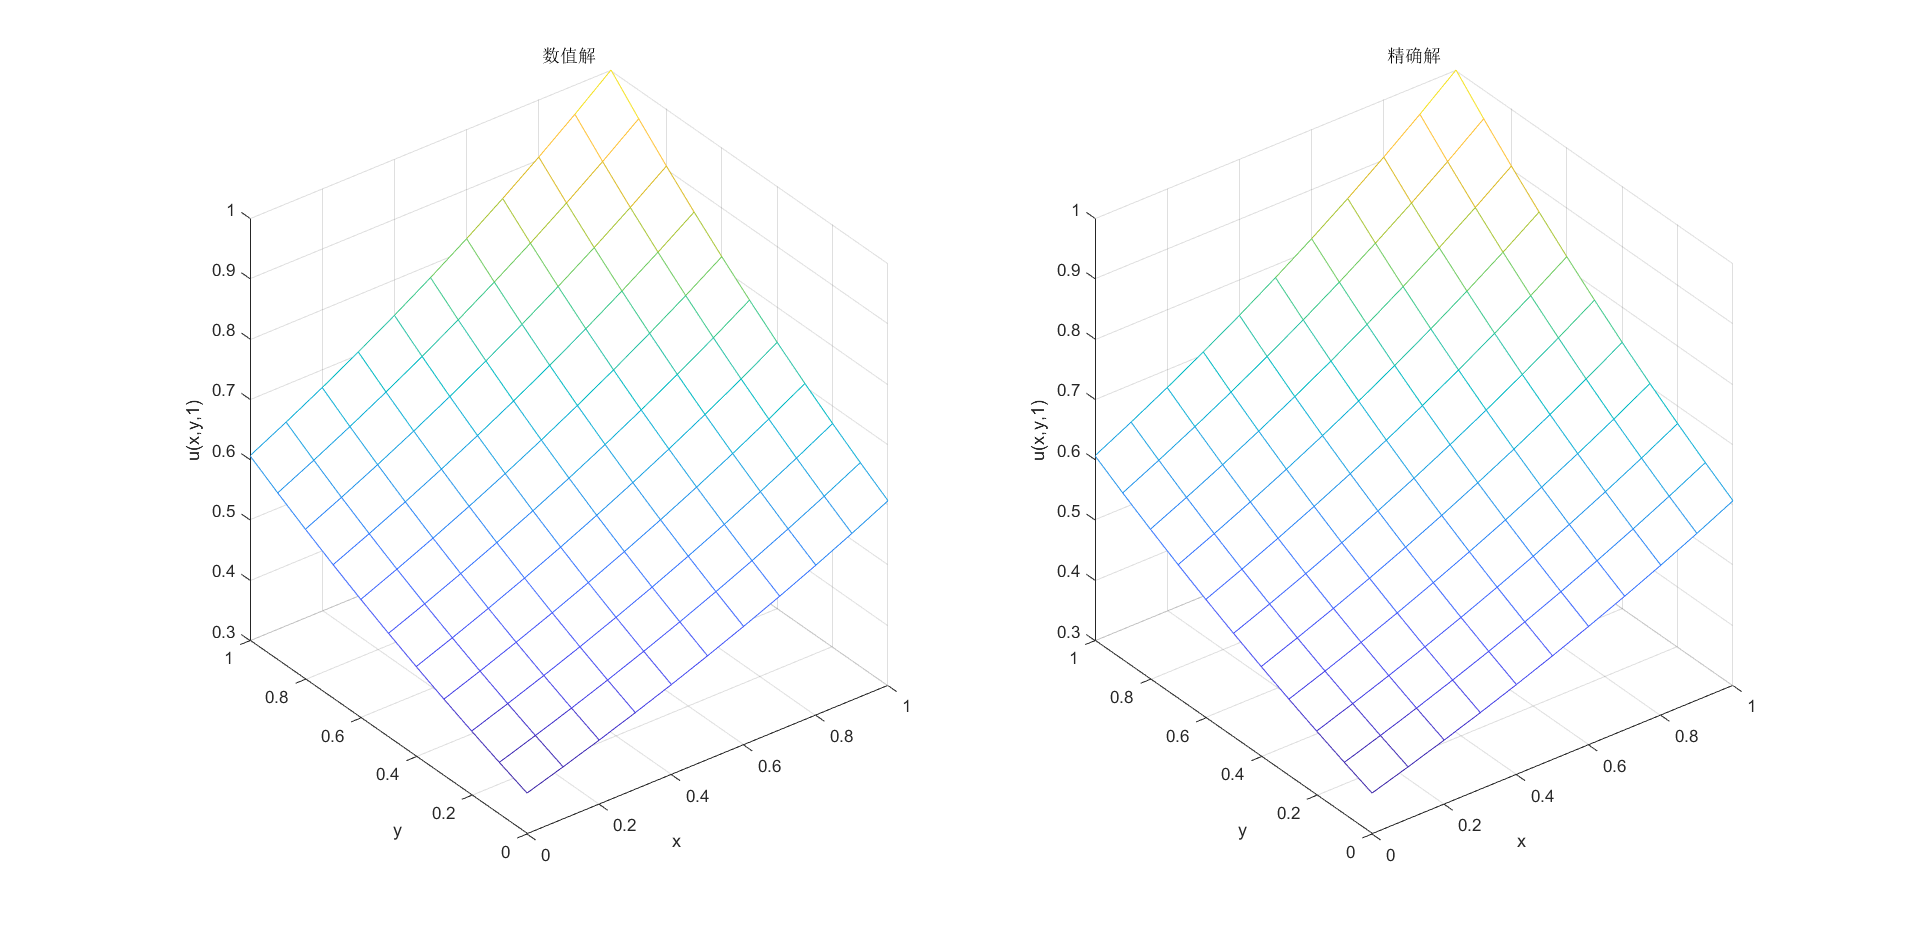
\includegraphics[width=1\linewidth]{figures/f1}
	\caption{$\tau=\dfrac{1}{100},h=\dfrac{1}{10}$时t=1处的数值解和精确解}
	\label{fig:f1}
\end{figure}

部分节点处的数值解、精确解和误差见表\ref{tab:1}.
% Table generated by Excel2LaTeX from sheet 'Sheet1'
\begin{table}[htbp]
	\centering
	\caption{部分节点处的数值解、精确解和误差}
	\begin{tabular}{cccc}
		\toprule[1.5pt]
		t,x,y & 数值解   & 精确解   & 误差 \\
		\midrule[1pt]
		0.1,0.5,0.5 & 1.492229  & 1.491825  & 4.0480E-04 \\
		0.2,0.5,0.5 & 1.350296  & 1.349859  & 4.3716E-04 \\
		0.3,0.5,0.5 & 1.221809  & 1.221403  & 4.0652E-04 \\
		0.4,0.5,0.5 & 1.105540  & 1.105171  & 3.6952E-04 \\
		0.5,0.5,0.5 & 1.000335  & 1.000000  & 3.3462E-04 \\
		0.6,0.5,0.5 & 0.905140  & 0.904837  & 3.0282E-04 \\
		0.7,0.5,0.5 & 0.819005  & 0.818731  & 2.7401E-04 \\
		0.8,0.5,0.5 & 0.741066  & 0.740818  & 2.4793E-04 \\
		0.9,0.5,0.5 & 0.670544  & 0.670320  & 2.2434E-04 \\
		1.0,0.5,0.5 & 0.606734  & 0.606531  & 2.0299E-04 \\
		\bottomrule[1.5pt]
	\end{tabular}%
	\label{tab:1}%
\end{table}%

t=1时,取不同步长时的误差见图\ref{fig:2},步长越小,误差越小。
\begin{figure*}
	\centering
	\begin{subfigure}[b]{0.475\textwidth}
		\centering
		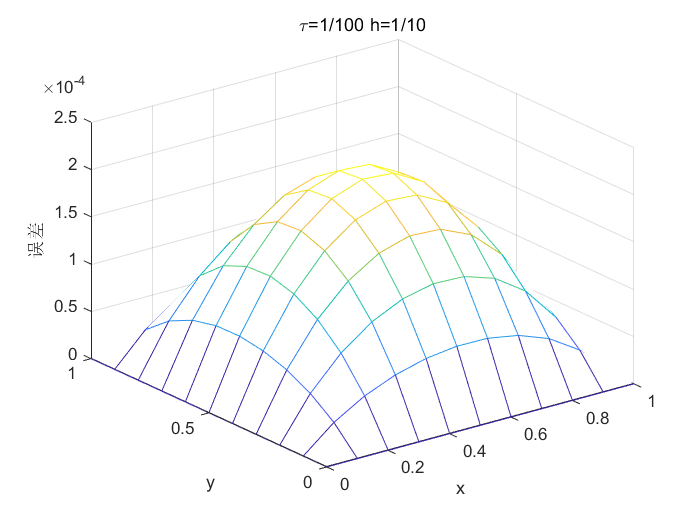
\includegraphics[width=\textwidth]{figures/f2}
		\caption[Network2]%
		{{\small $h=1/10,\tau=1/100$时的误差}}    
		\label{fig:mean and std of net14}
	\end{subfigure}
	\hfill
	\begin{subfigure}[b]{0.475\textwidth}  
		\centering 
		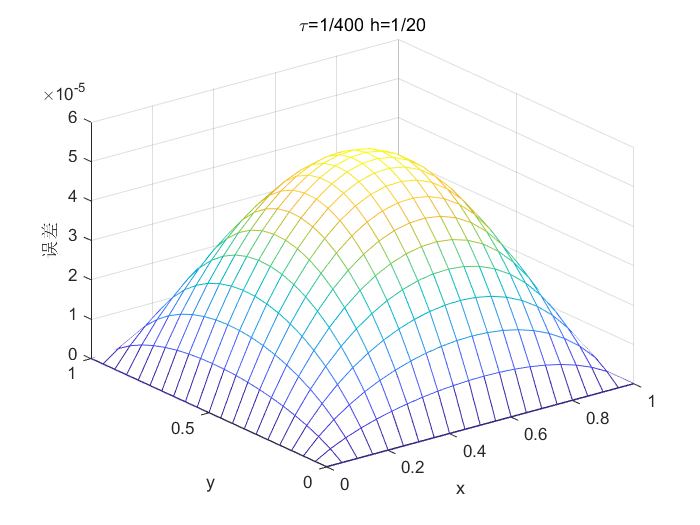
\includegraphics[width=\textwidth]{figures/f3}
		\caption[]%
		{{\small $h=1/20,\tau=1/400$时的误差}}    
		\label{fig:mean and std of net24}
	\end{subfigure}
	\vskip\baselineskip
	\begin{subfigure}[b]{0.475\textwidth}   
		\centering 
		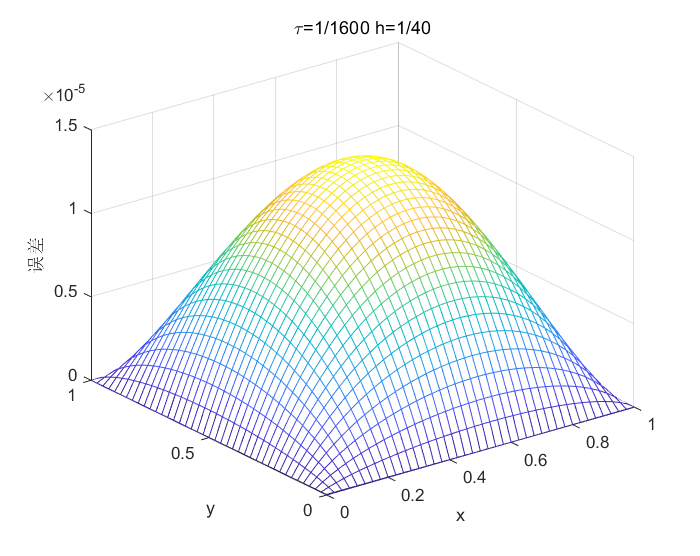
\includegraphics[width=\textwidth]{figures/f4}
		\caption[]%
		{{\small $h=1/40,\tau=1/1600$时的误差}}    
		\label{fig:mean and std of net34}
	\end{subfigure}
	\quad
	\begin{subfigure}[b]{0.475\textwidth}   
		\centering 
		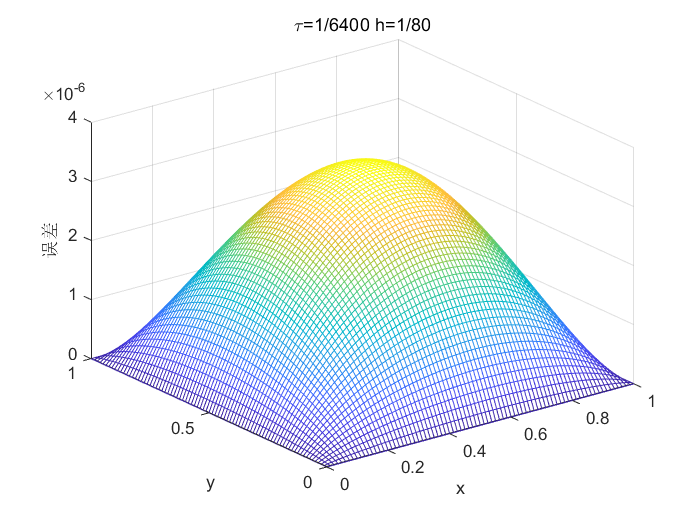
\includegraphics[width=\textwidth]{figures/f5}
		\caption[]%
		{{\small $h=1/180,\tau=1/6400$时的误差}}    
		\label{fig:mean and std of net44}
	\end{subfigure}
	\caption[ The average and standard deviation of critical parameters ]
	{t=1时的误差图} 
	\label{fig:2}
\end{figure*}
	
	取不同步长时的最大误差和最大误差的比见表\ref{tab:2},$h$变为原来的
	2倍,$\tau$变为原来的4倍,最大误差变为原来的4倍。
	% Table generated by Excel2LaTeX from sheet 'Sheet1'
	\begin{table}[htbp]
		\centering
		\caption{不同步长时的最大误差和最大误差的比}
		\begin{tabular}{ccc}
			\toprule[1.5pt]
			$h,\tau$   & $E_{\infty}(h,\tau)$ & $E_{\infty}(2h,2\tau)/E_{\infty}(h,\tau)$ \\
			\midrule[1pt]
			1/10,1/100 & 4.40E-04 & * \\
			1/20,1/400 & 1.16E-04 & 3.7873  \\
			1/40,1/1600 & 2.94E-05 & 3.9525  \\
			1/80,1/6400 & 7.38E-06 & 3.9842  \\
			\bottomrule[1.5pt]
		\end{tabular}%
		\label{tab:2}%
	\end{table}%
	

\end{document}